\section{GNSS}
\subsection{Coordenadas Geográficas}
    \begin{frame}{Coordenadas Geográficas}
        \begin{columns}
            \begin{column}{0.55\textwidth}
                \centering
                \begin{tikzpicture}[scale=1,tdplot_main_coords,every node/.style={font = {\footnotesize}}]
% https://latex.org/forum/viewtopic.php?t=25316

\def\rvec{3.5}

\def\phivecA{30}
\def\thetavecA{75}

\def\phivecB{45}
\def\thetavecB{17.5}

\def\auxOpacity{0.75}

\pgfmathsetmacro{\ax}{\rvec*sin(\phivecA)*cos(\thetavecA)}
\pgfmathsetmacro{\ay}{\rvec*sin(\phivecA)*sin(\thetavecA)}
\pgfmathsetmacro{\az}{\rvec*cos(\phivecA)}
\pgfmathsetmacro{\ac}{\rvec*sin(\phivecA)}

\pgfmathsetmacro{\bx}{\rvec*sin(\phivecB)*cos(\thetavecB)}
\pgfmathsetmacro{\by}{\rvec*sin(\phivecB)*sin(\thetavecB)}
\pgfmathsetmacro{\bz}{\rvec*cos(\phivecB)}
\pgfmathsetmacro{\bc}{\rvec*sin(\phivecB)}


\shadedraw[tdplot_screen_coords, ball color = white, opacity=0.25] (0,0) circle (\rvec);

%-----------------------
\coordinate (O) at (0,0,0);

\tdplotsetcoord{A}{\rvec}{\phivecA}{\thetavecA}

\tdplotsetcoord{B}{\rvec}{\phivecB}{\thetavecB}

\tdplotsetcoord{N}{\rvec}{0}{90}

%draw the main coordinate system axes
\draw[thick,-latex] (O) -- (1.35*\rvec,0,0) node[anchor=north east]{$x$};
\draw[thick,-latex] (O) -- (0,1.35*\rvec,0) node[anchor=north west]{$y$};
\draw[thick,-latex] (O) -- (0,0,1.35*\rvec) node[anchor=south]{$z$};

\draw[thick,-latex,opacity=0] (O) -- (-1.35*\rvec,0,0) node[anchor=south west]{$x$};
\draw[thick,-latex,opacity=0] (O) -- (0,-1.35*\rvec,0) node[anchor=south east]{$y$};
\draw[thick,-latex,opacity=0] (O) -- (0,0,-1.35*\rvec) node[anchor=north]{$z$};


\draw[-latex,very thick,opacity=\auxOpacity, color=Green] (O) -- (A) node[anchor=south west, opacity=1] {$\mathbf{A}_\text{g}$};
\draw[-latex,very thick,opacity=\auxOpacity, color=Blue] (O) -- (B) node[anchor=south east, opacity=1] {$\mathbf{A}_\text{g}$};
\draw[very thick,color=Black] (N) node[anchor=west] {$\mathbf{N}$};


\draw[dashed, opacity=0.15] (\rvec,0,0) arc (0:360:\rvec);
\draw[thin] (\rvec,0,0) arc (0:135:\rvec);
\draw[thin] (\rvec,0,0) arc (0:-45:\rvec);

\draw[dashed, color=Green, opacity=\auxOpacity] (O) -- (Axy) -- (A);
\draw[dashed, color=Blue, opacity=\auxOpacity] (O) -- (Bxy) -- (B);

\draw[dotted, color=Green, opacity=\auxOpacity] (Ax) -- (Axy);
\draw[dotted, color=Green, opacity=\auxOpacity] (Ay) -- (Axy);

\draw[dotted, color=Blue, opacity=\auxOpacity] (Bx) -- (Bxy);
\draw[dotted, color=Blue, opacity=\auxOpacity] (By) -- (Bxy);

\pause


\tdplotdrawarc[color=Green, opacity=\auxOpacity]{(O)}{\ac}{0}{\thetavecA}{anchor=north}{$\theta_{\mathbf{A}_\text{g}}$}

\tdplotdrawarc[color=Blue, opacity=\auxOpacity]{(O)}{\bc}{0}{\thetavecB}{anchor=north east}{$\theta_{\mathbf{B}_\text{g}}$}

\pause


\tdplotsetthetaplanecoords{\thetavecA}
\tdplotdrawarc[color=Green, opacity=\auxOpacity, tdplot_rotated_coords]{(O)}{\ac}{90}{\phivecA}{anchor=west}{$\phi{\mathbf{A}_\text{g}}$}

\tdplotsetthetaplanecoords{\thetavecB}
\tdplotdrawarc[color=Blue, opacity=\auxOpacity, tdplot_rotated_coords]{(O)}{\bc}{90}{\phivecB}{anchor=east}{$\phi{\mathbf{B}_\text{g}}$}

\pause

\tdplotsetthetaplanecoords{\thetavecB}
\draw[dashed, Blue, opacity=0.15, tdplot_rotated_coords] (\rvec,0,0) arc (180:-40:-\rvec);
\draw[thin, Blue, opacity=0.25, tdplot_rotated_coords] (\rvec,0,0) arc (0:140:\rvec);
\draw[thin, Blue, opacity=0.25, tdplot_rotated_coords] (\rvec,0,0) arc (360:320:\rvec);
\draw[very thick, color=Blue, tdplot_rotated_coords] (\rvec,0,0) arc (0:\phivecB:\rvec);

\tdplotsetthetaplanecoords{\thetavecA}
\draw[dashed, Green, opacity=0.15, tdplot_rotated_coords] (\rvec,0,0) arc (180:-40:-\rvec);
\draw[thin, Green, opacity=0.25, tdplot_rotated_coords] (\rvec,0,0) arc (0:140:\rvec);
\draw[thin, Green, opacity=0.25, tdplot_rotated_coords] (\rvec,0,0) arc (360:320:\rvec);
\draw[very thick, color=Green, tdplot_rotated_coords] (\rvec,0,0) arc (0:\phivecA:\rvec);


\drawArc{\ax}{\ay}{\az}{\bx}{\by}{\bz}{\rvec}{anchor=north}{$d_\mathbf{AB}$}

\tdplotsetrotatedcoords{\phivecA}{\thetavecA}{0}

\def\centerarc[#1](#2)(#3:#4:#5)% Syntax: [draw options] (center) (initial angle:final angle:radius)
    { \draw[#1] ($(#2)+({#5*cos(#3)},{#5*sin(#3)})$) arc (#3:#4:#5) node[midway,anchor=south east] {$\beta_b$}; }

\centerarc[Red, tdplot_rotated_coords](A)(292:214:0.4)

\end{tikzpicture}
                % 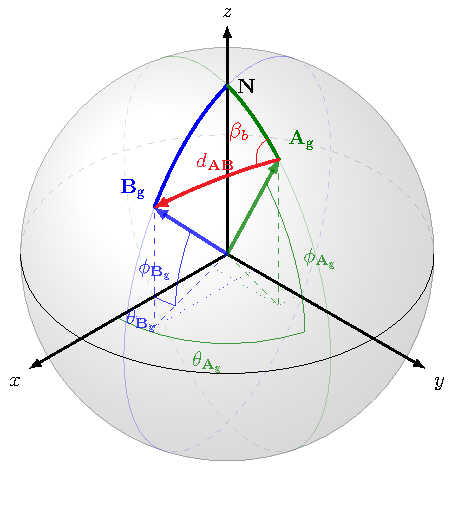
\includegraphics[width=0.95\textwidth]{../pictures/globo.pdf}
            \end{column}
            \begin{column}{0.45\textwidth}
                \begin{itemize}[<+(-3)->]\addtolength{\itemsep}{0.5\baselineskip}
                    \item \textcolor{Green}{$\mathbf{A}_\text{g}$} e \textcolor{Blue}{$\mathbf{B}_\text{g}$} são coordenadas geográficas
                    \item \textcolor{Green}{$\theta_{\mathbf{A}_\text{g}}$} e \textcolor{Blue}{$\theta_{\mathbf{B}_\text{g}}$} são latitudes
                    \item \textcolor{Green}{$\phi_{\mathbf{A}_\text{g}}$} e \textcolor{Blue}{$\phi_{\mathbf{B}_\text{g}}$} são longitudes
                    \item Conhecendo essas informações, é possível determinar o ângulo \textcolor{Red}{$\beta_b$} relativo entre as duas coordenadas
                    \item Também é possível determinar sua distância \textcolor{Red}{$d_\mathbf{AB}$}
                \end{itemize}
            \end{column}
        \end{columns}
    \end{frame}

% \subsection{Cálculo de Bearing}
%     \begin{frame}{Cálculo de Bearing}
%         % \begin{multicols}{2}
%             \begin{equation*}
%                 \Delta_\phi = \textcolor{Blue}{\phi_{\mathbf{B}_\text{g}}} - \textcolor{Green}{\phi_{\mathbf{A}_\text{g}}}
%             \end{equation*}
%             \begin{equation*}
%                 \Delta_\theta = \textcolor{Blue}{\theta_{\mathbf{B}_\text{g}}} - \textcolor{Green}{\theta_{\mathbf{A}_\text{g}}}
%             \end{equation*}
%             \begin{equation*}
%                 X = \cos\left(\textcolor{Blue}{\theta_{\mathbf{B}_\text{g}}}\right)\cdot \sin\left(\Delta_\phi\right)
%             \end{equation*}
%             \begin{equation*}
%                 Y = \cos\left(\textcolor{Green}{\theta_{\mathbf{A}_\text{g}}}\right)\cdot\sin\left(\textcolor{Blue}{\theta_{\mathbf{B}_\text{g}}}\right) - \sin\left(\textcolor{Green}{\theta_{\mathbf{A}_\text{g}}}\right) \cdot \cos\left(\textcolor{Green}{\theta_{\mathbf{B}_\text{g}}}\right) \cdot \cos\left(\Delta_\phi\right)
%             \end{equation*}
%             \begin{equation*}
%                 Z = \sin^2\left(\frac{\Delta_\theta}{2}\right) + \cos\left(\textcolor{Blue}{\theta_{\mathbf{B}_\text{g}}}\right) \cdot \cos\left(\textcolor{Green}{\theta_{\mathbf{A}_\text{g}}}\right) \cdot \sin^2\left(\frac{\Delta_\phi}{2}\right)
%             \end{equation*}
%             \begin{equation*}
%                 \textcolor{Red}{\beta_b} = \arctan\left(\frac{X}{Y}\right) - \frac{\pi}{2}
%             \end{equation*}
%             \begin{equation*}
%                 \textcolor{Red}{d_\mathbf{AB}} = R_\text{Terra} \cdot 2 \cdot \arctan\left(\frac{\sqrt{Z}}{\sqrt{1-Z}}\right)
%             \end{equation*}
%         % \end{multicols}
%     \end{frame}

\begin{frame}{Coordenadas Geográficas}
	\begin{itemize}[<+->]\addtolength{\itemsep}{0.5\baselineskip}
		\item É necessário decodificar os dados recebidos pela telemetria do foguete;
		\item A precisão da busca fica dependente da precisão do GNSS;
		\item O método baseia-se na ideia de que a equipe de busca tem acesso à própria coordenada geográfica;
		\item Num espaço sem acesso à internet, obter tal coordenada pode ser um problema;
		\item Se o sinal da telemetria for fraco, pode se tornar inviável utilizar este método.
	\end{itemize}
\end{frame}
